% Introduction to the solvers in ug4

\documentclass[xcolor=dvipsnames]{beamer}

\usepackage[latin1]{inputenc}
\usepackage{amsmath, amsfonts, amssymb}
\usepackage{graphicx}
\usepackage{color}
\usepackage{setspace}

\usetheme{Copenhagen}
\usecolortheme[named=YellowOrange]{structure}

%\usefonttheme{default}
\usefonttheme {structurebold}
\useinnertheme{default}
\useoutertheme{default}
\setbeamertemplate{headline}[default]

\newcommand*\oldmacro{}%
\let\oldmacro\insertshorttitle%
\renewcommand*\insertshorttitle{%
  \oldmacro\hfill%
  \insertframenumber\,/\,\inserttotalframenumber}

\title
 [ug4: Solvers]
 {Solvers in ug4}
\author [D. Logashenko] {Dmitry Logashenko}
\institute [CEMSE]
{CEMSE, KAUST, Saudi Arabia}
\date [Feb. 2025] {February 2025}

\begin{document}

\frame {\titlepage}

\begin {frame} [t]
\frametitle {Contents}
\tableofcontents
\end {frame}

\section {Linear solvers}

\begin {frame} [t]
\frametitle {Large sparse linear systems}
The discretization results in the system
$$
	\mathbf{A} \mathbf{u} = \mathbf{f}, \qquad \mathbf{A} \in \mathbb{R}^{n \times n}, \, u, f \in \mathbb{R}^n.
$$
\vspace {-3ex}
\begin {itemize}
	\pause
	\item $\mathbf{A}$ is {\color{blue} sparse} (only few non-zeros per row).
		But {\color{blue}for large $n$, direct solvers become inefficient}
		(their computational cost and memory requirements grow
		very rapidly with $n$).
	\pause
	\item Remedy: {\color{blue} Iterative methods}, computing
		$$
			\mathbf{u}^{(0)}, \mathbf{u}^{(1)}, \dots, \mathbf{u}^{(s)}, \mathbf{u}^{(s+1)}, \dots \to \mathbf{u}
		$$
		by for ex.\ the linear iteration
		$$
			\mathbf{u}^{(s+1)} = \mathbf{u}^{(s)} + \mathbf{W}^{-1} (\mathbf{f} - \mathbf{A} \mathbf{u}^{(s)})
		$$
		with a {\color{blue} preconditioner} $\mathbf{W}$ that approximates $\mathbf{A}$.
\end {itemize}
\end {frame}

\begin {frame} [t]
\frametitle {Efficient linear solvers}
\vspace {-2ex}
\begin {itemize}
	\item The Gaussian elimination can be {\color{blue} efficient for relatively coarse grids}
		(a couple of thousand of degrees of freedom).
	\pause
	\item Efficiency of linear and non-linear (CG, BiCGStab, GMRES etc.) iterations
		depends essentially on {\color{blue} the preconditioner}. Convergence rate of simple preconditioners
		(Jacobi, Gauss-Seidel, ILU) {\color{blue} deteriorates for big $n$} (i.e. small $h$). Reason:
		Slow damping of low-frequency modes in the error.
	\pause
	\item {\color{blue} Multigrid methods} achieve mesh-size independent convergence rate.
		They use the s.c. coarse grid correction on a grid hierarchy for damping the low-frequency modes.
		On the coarsest grid, the system is solved by for ex.\ a direct solver ({\color{blue}
		coarse grid solver}), and on the other levels, simple preconditioners are used as
		{\color{blue} smoothers}.
	\pause
	\item Efficient iterative solvers can be sensitive to properties of the linear
		system ({\color{blue} robustness}).
\end {itemize}
\end {frame}

\begin {frame} [t]
\frametitle {Solver objects: A linear model}
\centerline {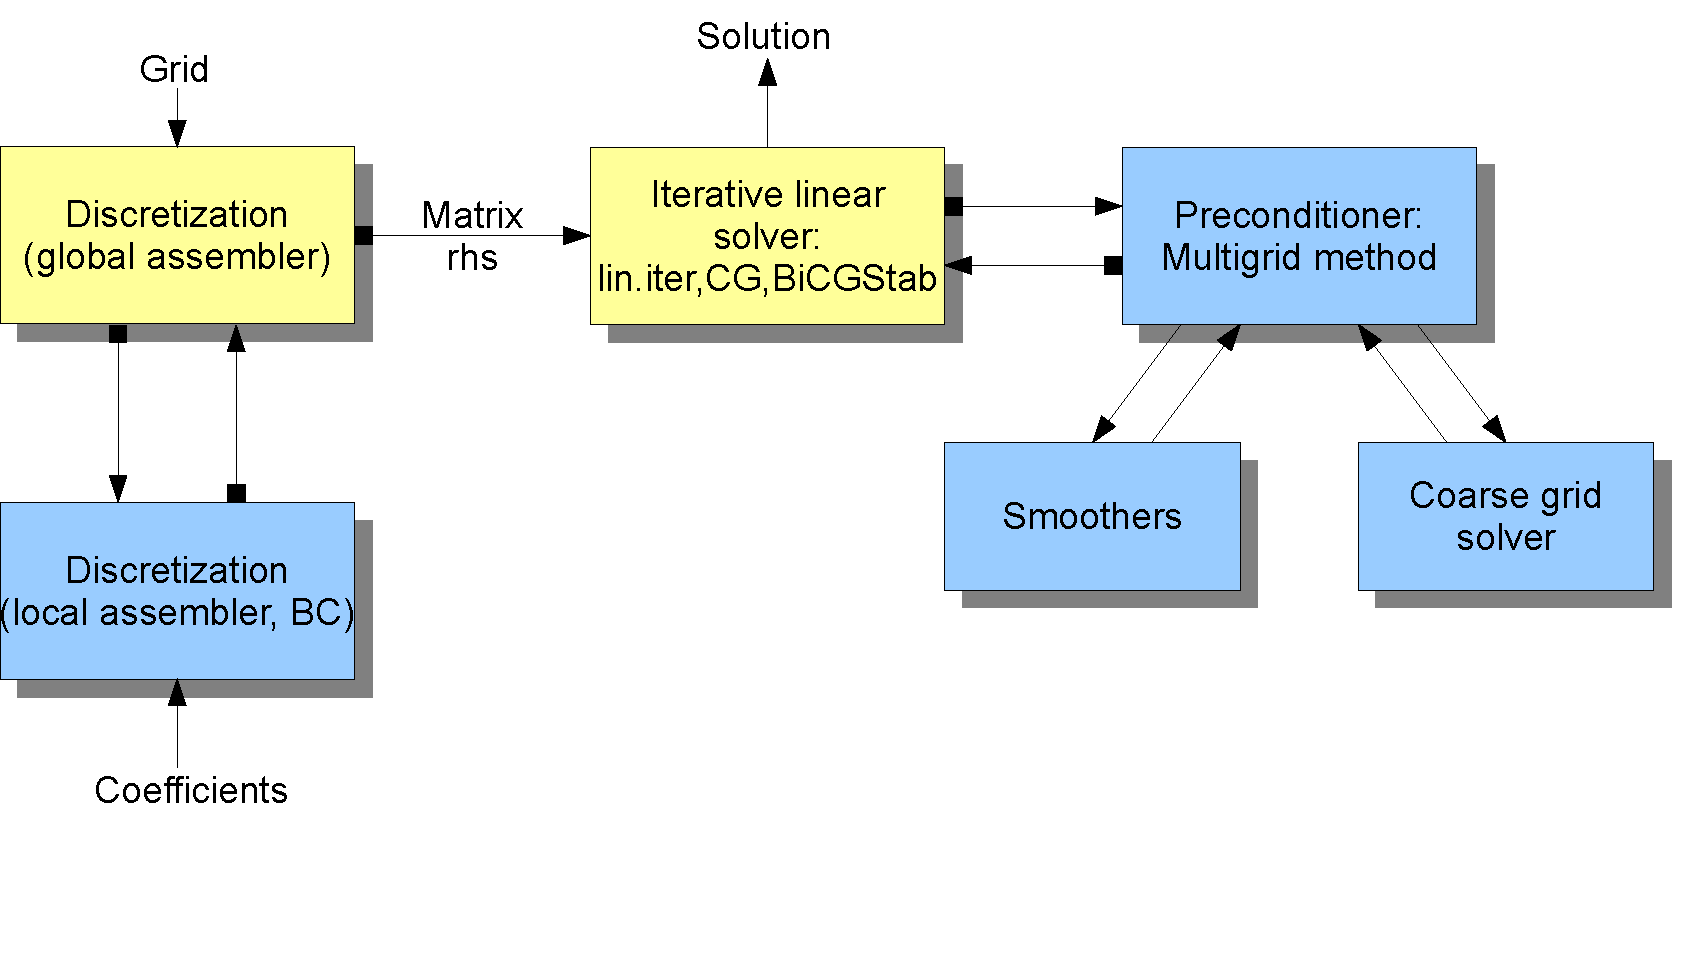
\includegraphics [width=1.15\textwidth] {LinearSolverFull}}
\end {frame}

\section {Non-linear solvers}

\begin{frame}
\frametitle{BVP for stationary incompressible NS}
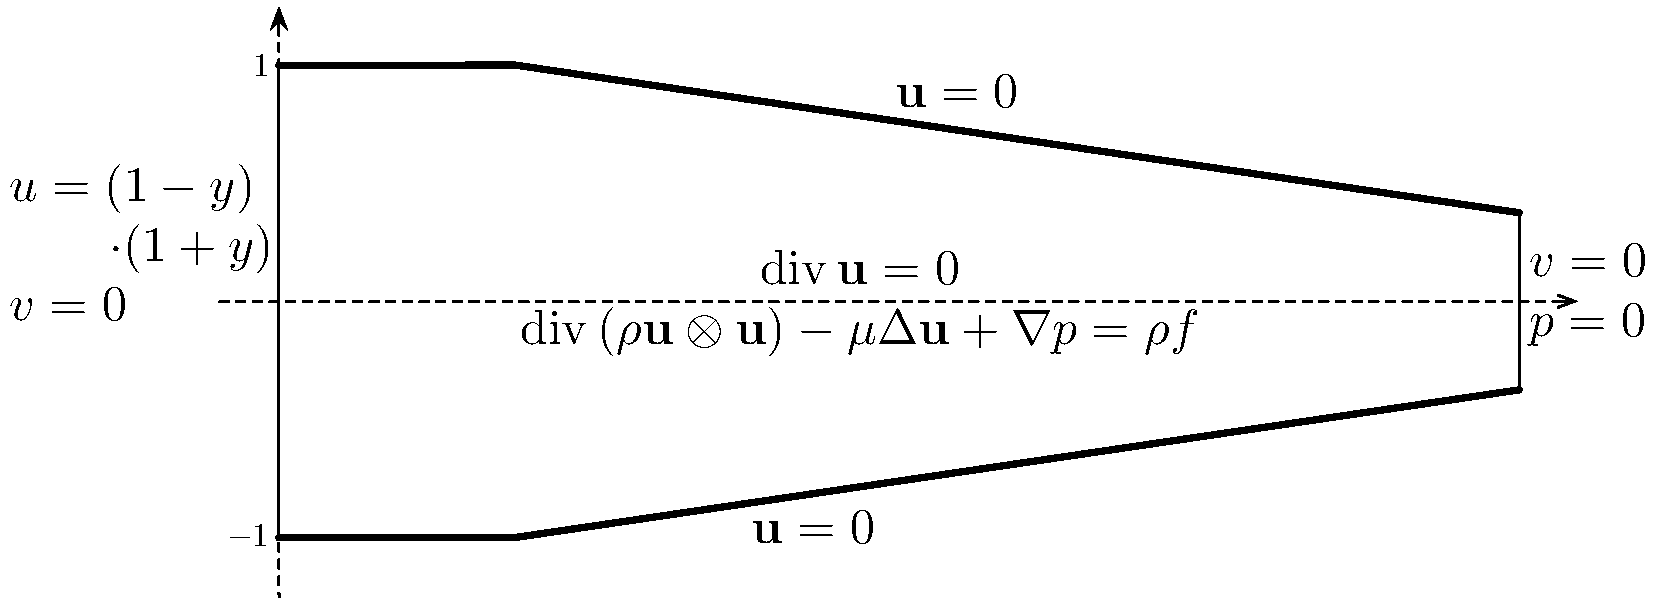
\includegraphics [width=\textwidth] {NSDuese.pdf}

\vspace {2ex}
\centerline {$d = 2$, $\mathbf{u} = (u, v)^T$}
\end{frame}

\begin {frame} [t]
\frametitle {Numerical solutions of the NS equations}
\begin {itemize}
	\item The incompressible Navier-Stokes equations constitute (for non-vanishing viscosity)
		a saddle-point system. The existence of the solution depends of the LBB (or inf-sup)
		condition.
	\pause
	\item The stability of the discretization depends on the discrete inf-sup condition
		which is not inherited from the continuous problem (unlike the ellipticity).
		This requires special discretization approaches (ex.: the staggered grids).
	\pause
	\item Coupling of the equations requires the ``pressure correction''
		(ex.: the SIMPLE method) or a stabilization.
	\pause
	\item The discretized saddle-point linear systems require special linear solvers.
	\pause
	\item ug4 implements a {\color{blue} stabilized collocated FV discretization}.
\end {itemize}
\end {frame}

\begin{frame} [t]
\frametitle {Non-linear equations}
Discretized {\color{blue} non-linear} algebraic system of algebraic equations on $\Omega_h$:
$$
 \mathcal{A} (u) = 0
$$
\begin{itemize}
 \pause
 \item {\color{blue} ``Sparse''}: Every equation depends only on a small number of DoFs for any $h$.
 \pause
 \item It may have {\color{blue} several solutions} $u$. However, typically it is assumed that $u$ is unique.
 \pause
 \item $\mathcal{A}$ should be differentiable at least in a neighbourhood of the solution.
\end{itemize}
\end{frame}

\begin{frame} [t]
\frametitle {Iterative non-linear solvers}
\dots compute a sequence
$$
 u_0, u_1, u_2, \dots, u_k, \dots
$$
that should converge to the solution $u_{*}$ of $\mathcal{A} (u) = 0$.

\pause
\vspace{2ex}
$d_k := \mathcal{A} (u_k)$ is said to be the \emph{defect} of $u_k$.

\pause
\vspace{2ex}
The system is linearized. We denote by $\mathbf{A}_k$ the Jacobian of
$\mathcal{A}$ at $u_k$. By $\tilde{\mathbf{A}}_k$, we denote its approximation, e.g.
$\tilde{\mathbf{A}}_k = \mathbf{A}_k$.

\pause
\vspace{2ex}
Typical iteration:
$$
 u_{k+1} = u_k - \alpha_k \tilde{\mathbf{A}}_k^{-1} \mathcal{A} (u_k)
$$
with \emph{step length} $\alpha_k$.
\end{frame}

\begin{frame} [t]
\frametitle {Implementation of the non-linear solvers}
\begin{itemize}
 \item The non-linear operator $\mathcal{A}$ {\color{blue} cannot be represented in the memory}.
 \pause
 \item Instead, one implements functions evaluating {\color{blue} grid function} $\mathcal{A} (u_k)$
  and the large sparse matrix $\tilde{\mathbf{A}}_k$ for every $u_k$.
 \pause
 \item To get $\tilde{\mathbf{A}}_k^{-1} \mathcal{A} (u_k)$, solve the system
  $$
   \tilde{\mathbf{A}}_k c_k = d_k
  $$
  (e.g. by the GMG method).
 \pause
 \item $\alpha_k$ is obtained by {\color{blue} linesearch}.
\end{itemize}
\end{frame}

\begin{frame} [t]
\frametitle {Linesearch}
For every $k$ we try
$$
 \alpha_k = \alpha_k^{(0)}, \alpha_k^{(1)}, \dots, \alpha_k^{(m)}
$$
with $\alpha_k^{(i+1)} = \alpha_k^{(i)} / \gamma$ (up to some prespecified $m$). Typically $\gamma = 2$.

\pause
\vspace{1ex}
For $\alpha_k$ take e.g.\ the first $\alpha_k^{(i)}$ with
$$
 \| \mathcal{A} \bigl ( u_k - \alpha_k^{(i)} \tilde{\mathbf{A}}_k^{-1} \mathcal{A} (u_k) \bigr ) \|
  < (1 - \varepsilon \alpha_k^{(i)}) \| \mathcal{A} (u_k) \|
$$
($\varepsilon$: ``sufficient descent''). Otherwise set $\alpha_k = \alpha_k^{(m)}$.

\pause
\vspace{1ex}
There are different linesearch strategies.
\end{frame}

\begin {frame} [t]
\frametitle {Solver objects: A non-linear model}
\centerline {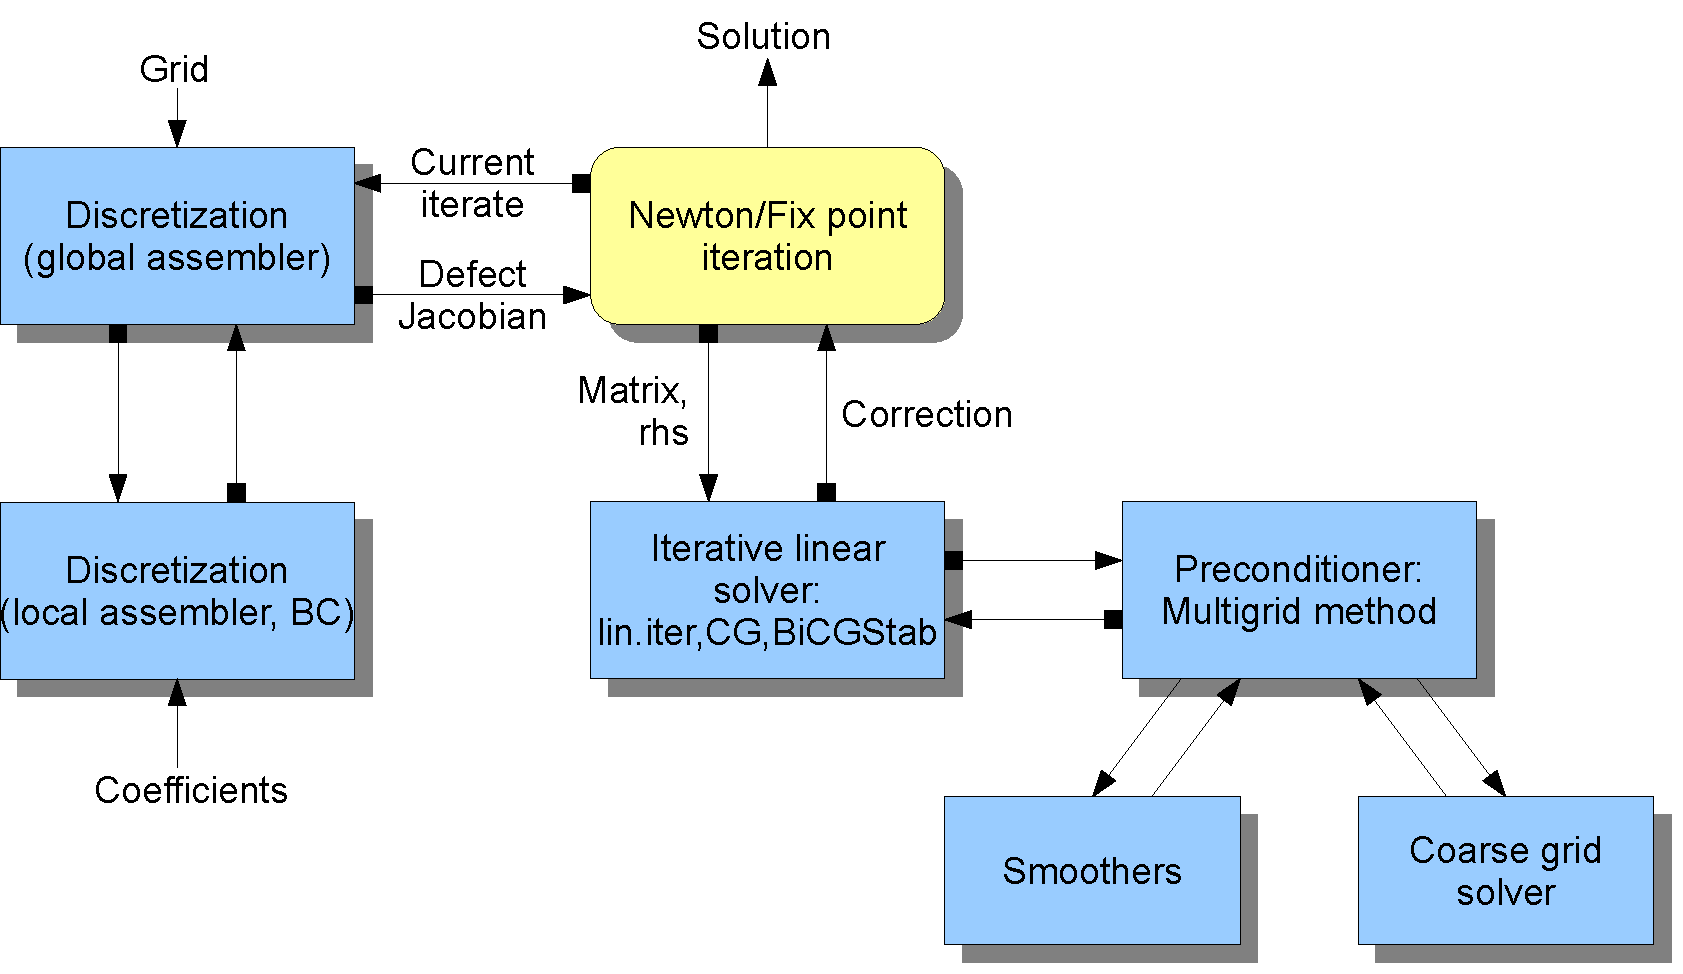
\includegraphics [width=1.15\textwidth] {StationarySolverFull}}
\end {frame}

\section {Objects of the numerical methods in ug4}

\begin {frame} [t]
\frametitle {Discretization and solver objects in ug4}
\vspace {-2ex}
\begin {itemize}
	\item Discretization and solvers are implemented as {\color{blue} classes}. The objects reference
		the subordinated objects (e.g. the GMG preconditioner references its smoothers and
		the coarse grid solver; the domain discretization references its element discretizations).
	\pause
	\item The objects are initialized with their parameters. For ex. the local discretizations
		are initialized with the problem coefficients. They can be represented in particular
		by the s.c. {\color{blue} user data} objects that may refer to e.g. LUA functions.
		(Note however that massive evaluation of LUA functions may reduce efficiency.)
	\pause
	\item The flexible hierarchy of the classes includes some auxiliary classes, in particular
		to specify the termination criteria for iterative methods or, for ex., the
		line search strategy for the Newton's method.
\end {itemize}
\end {frame}

\section {Conclusions}

\begin {frame} [t]
\frametitle {Thank you for your attention!}
We considered:
\begin {itemize}
	\item Sparse matrices and linear solvers in ug4
	\item Non-linear problems and non-linear solvers in ug4
\end {itemize}

\vspace{6ex}
Supplementary scripts:
\begin {itemize}
	\item poisson\_raw.lua --- setting up the linear solver for the Poisson equation
	\item stripe\_diff.lua --- solving a more general diffusion problem (with jumping diffusion coefficients)
	\item ns.lua --- solution of the Navier-Stokes problem (the ``cylinder'' example, a non-linear problem)
\end {itemize}
\end {frame}

\end{document}

% End of File
